\documentclass{beamer}
\usepackage{beamerthemesplit}
\usepackage{wrapfig}
\usetheme{SPbGU}
\usepackage{pdfpages}
\usepackage{amsmath}
\usepackage{cmap} 
\usepackage[T2A]{fontenc} 
\usepackage[utf8]{inputenc}
\usepackage[english,russian]{babel}
\usepackage{indentfirst}
\usepackage{amsmath}
\usepackage{tikz}
\usepackage{multirow}
\usepackage[noend]{algpseudocode}
\usepackage{algorithm}
\usepackage{algorithmicx}
\usetikzlibrary{shapes,arrows}
\usepackage{fancyvrb}
\usepackage{tikz}
\usepackage{pgfplots}
\usetikzlibrary{calc}
\usetikzlibrary{shapes,arrows}
\usetikzlibrary{arrows,automata}
\usetikzlibrary{positioning}
\usepackage[labelformat=empty]{caption}
\usepackage[labelformat=empty]{subcaption}
\beamertemplatenavigationsymbolsempty
\usepackage{multirow}
\usepackage{verbatim}
\usepackage{array}
\usepackage{graphicx}
\usepackage{multirow} 
\usepackage{fancyvrb}
\usepackage[misc,geometry]{ifsym} 
\newcolumntype{P}[1]{>{\centering\arraybackslash}p{#1}}


\newcommand{\tikzmark}[1]{\tikz[overlay,remember picture] \node (#1) {};}
\def\Put(#1,#2)#3{\leavevmode\makebox(0,0){\put(#1,#2){#3}}}

\newcommand{\ltz}{$< 1$}
\tikzset{
    state/.style={
           rectangle,
           rounded corners,
           draw=black, very thick,
           minimum height=2em,
           inner sep=4pt,
           text centered,
           },
}

\title[ФГ + НС]{Формальные грамматики и искусственные нейронные сети для предсказания вторичной структкры РНК}
\institute[]{
JetBrains Research, Programming Languages and Tools Lab \\
Санкт-Петербургский государственный университет }

\author[Полина Лунина]{Полина Лунина}


\date{19 декабря 2020г.}
\begin{document}
{
\begin{frame}[fragile]
  \begin{tabular}{p{2.0cm} p{7.5cm} p{1cm}}
   \begin{center}
      
\includegraphics[height=1.5cm]{pics/jetbrainsResearch.pdf}
    \end{center}
    &
    \begin{center}
      
\includegraphics[height=1.5cm]{pics/YC_logo.pdf}
    \end{center}
    &
    \begin{center}
      
\includegraphics[height=1.5cm]{pics/SPbGU_Logo.png}
    \end{center}
  \end{tabular}
  \titlepage
\end{frame}
}

\begin{frame} \frametitle{Биоинформатика}
\begin{tabular}{cl}  
    \parbox{0.44\linewidth}{
        \begin{itemize}
            \item Задачи
            \begin{itemize}
                \item Распознавание
                \item Классификация
                \item Предсказание вторичных структур
                \item ...
            \end{itemize}
  \onslide<2,3> {\item Формальное задание вторичной структуры}
  \onslide<3>  {\item Вероятностная оценка}
        \end{itemize}
    }
    & \begin{tabular}{l}
        \vspace{-0.8cm}
        \hspace{-0.8cm}
        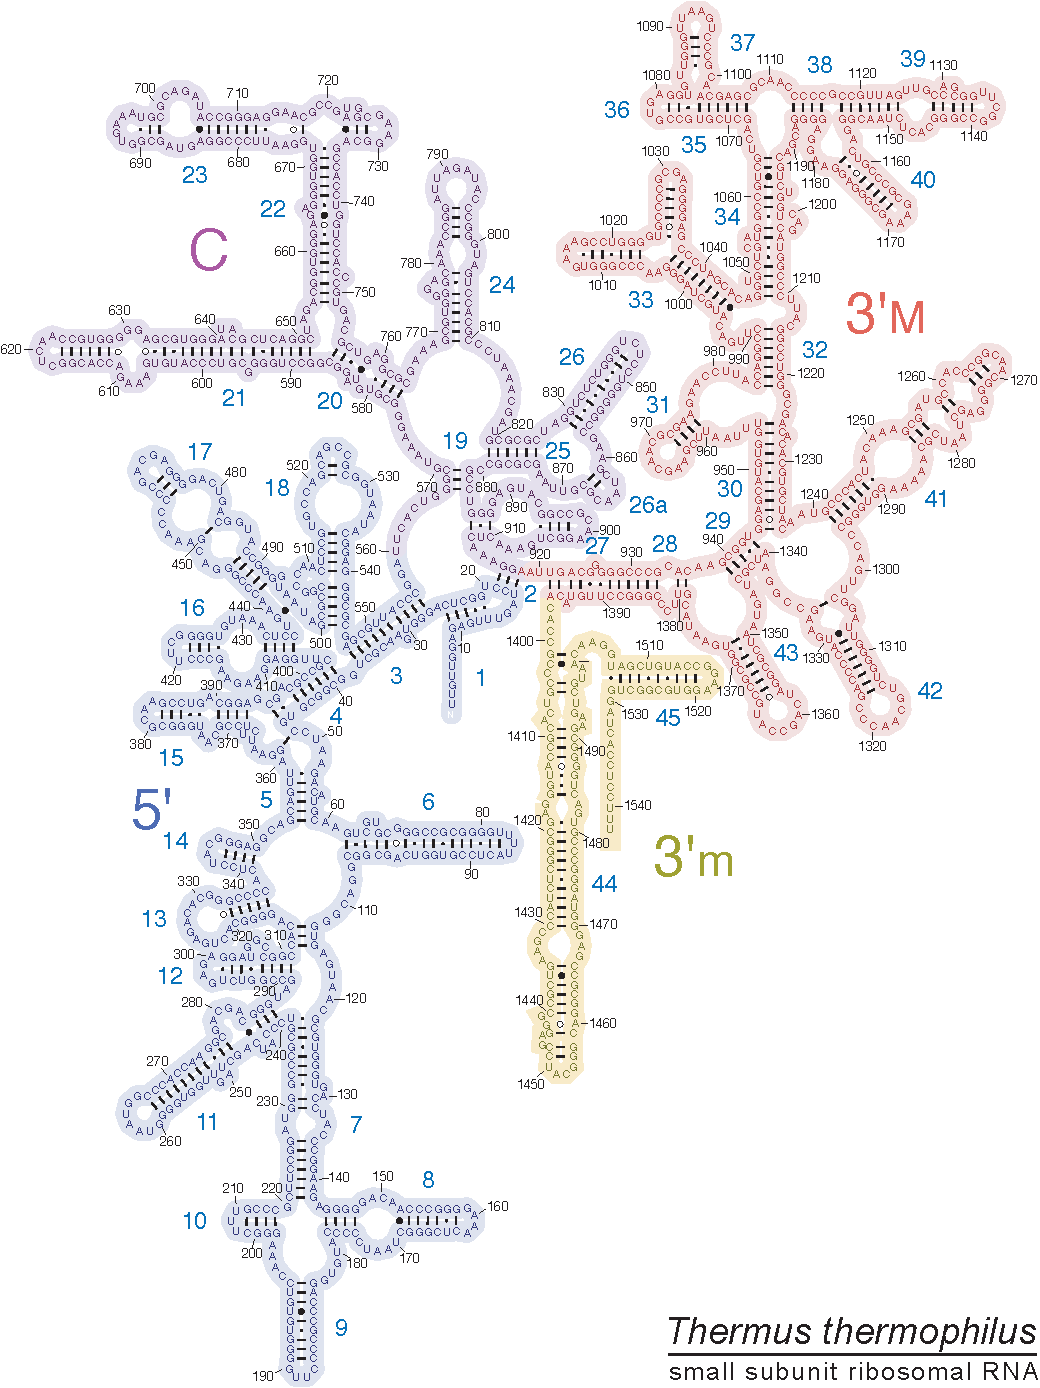
\includegraphics[width=5.0cm]{pics/16s.pdf}
    \end{tabular}  \\
\end{tabular}
\end{frame}


\begin{frame}{Подход: синтаксический анализ + машинное обучение}
\begin{itemize}
    \item Задать основные элементы вторичной структуры (стемы) с помощью грамматики 
    \item Искать стемы во входных цепочках при помощи парсера
    \item Для дальнейшей обработки и вероятностной оценки использовать нейронные сети
\end{itemize}

\vspace{1.0cm}
\begin{center}
    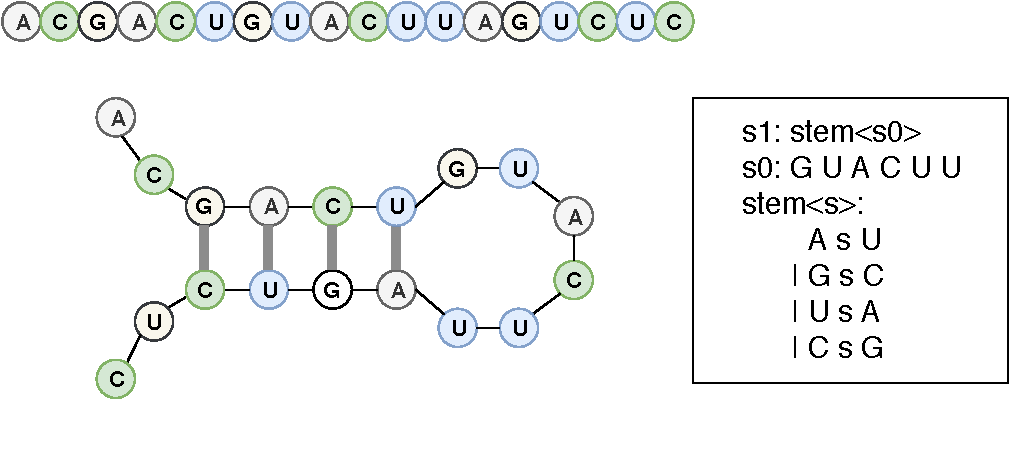
\includegraphics[width=9.5cm]{pics/molekula.pdf} 
\end{center}
    
\end{frame}




\begin{frame}{Пример}
\centering
 \texttt{CCCC{\color{red}AUUGCCAAGG}ACCCCA{\color{red}CCUUGGCAAU}CCC}
\vspace{1cm}

\tikzmark{xx}{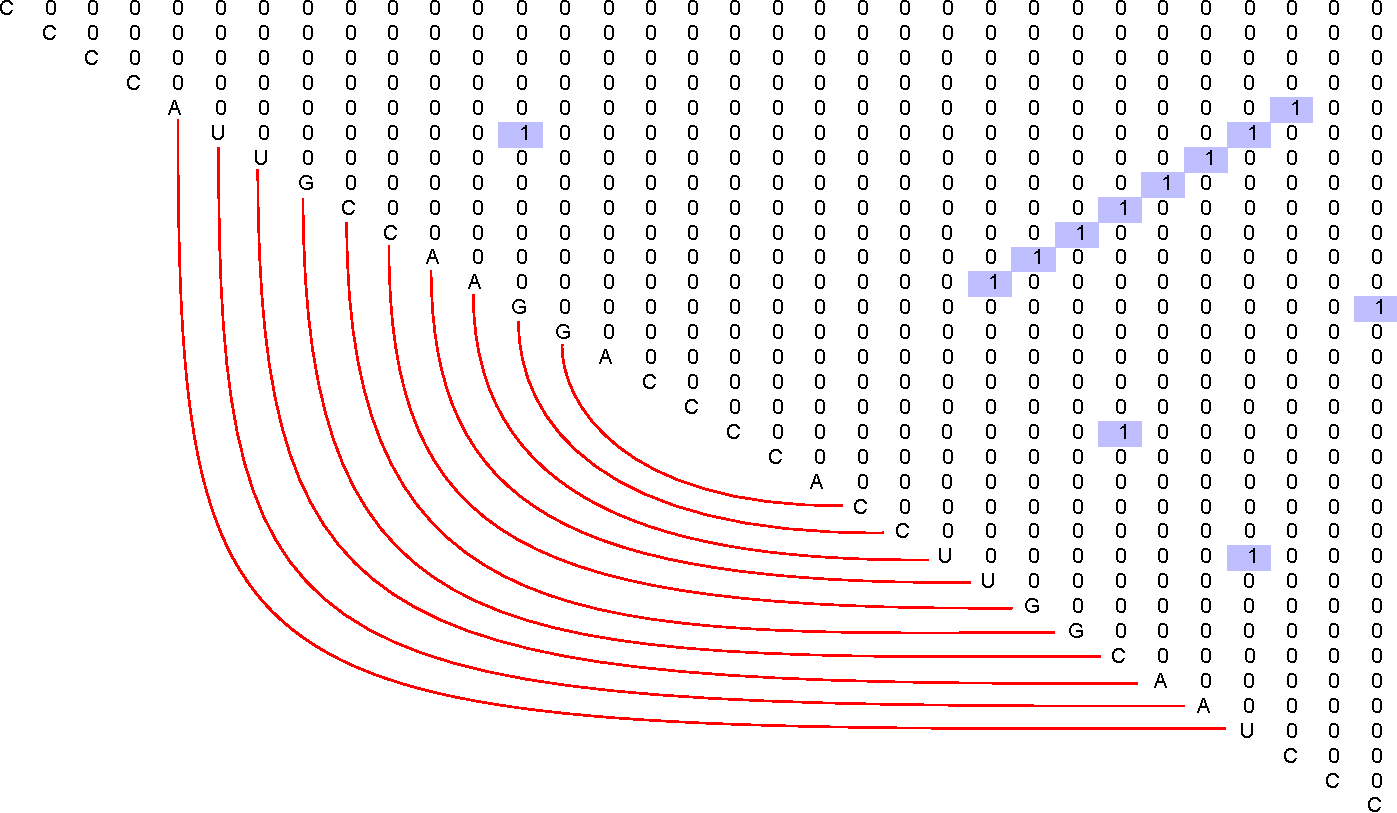
\includegraphics[width=.8\textwidth]{pics/mtr.pdf}}
\onslide<2-3>{
\tikz[overlay,remember picture]{
\draw[draw=red,thick,fill opacity=0.2] ($(xx) + (1.1,4.97)$) rectangle ($(xx) + (9.05,3.235)$);
}
}

\onslide<3>{
\tikz[overlay,remember picture]{
\draw[draw=red,thick,fill opacity=0.2] ($(xx) + (5.8,4.97)$) rectangle ($(xx) + (8.75,0.4)$);
}
}
\end{frame}



\begin{frame}{Предсказание вторичной структуры РНК} 
\begin{itemize}
    \item Парсер находит в цепочке все возможные стемы, однако не все они действительно будут входить в состав вторичной структуры
    \item Хотим отбработать матрицу разбора нейронной сетью и предсказать вторичную структуру цепочки
\end{itemize}
\vspace{0.5cm}
\begin{figure}
\centering
\begin{subfigure}{.3\textwidth}
  \centering
  \fbox{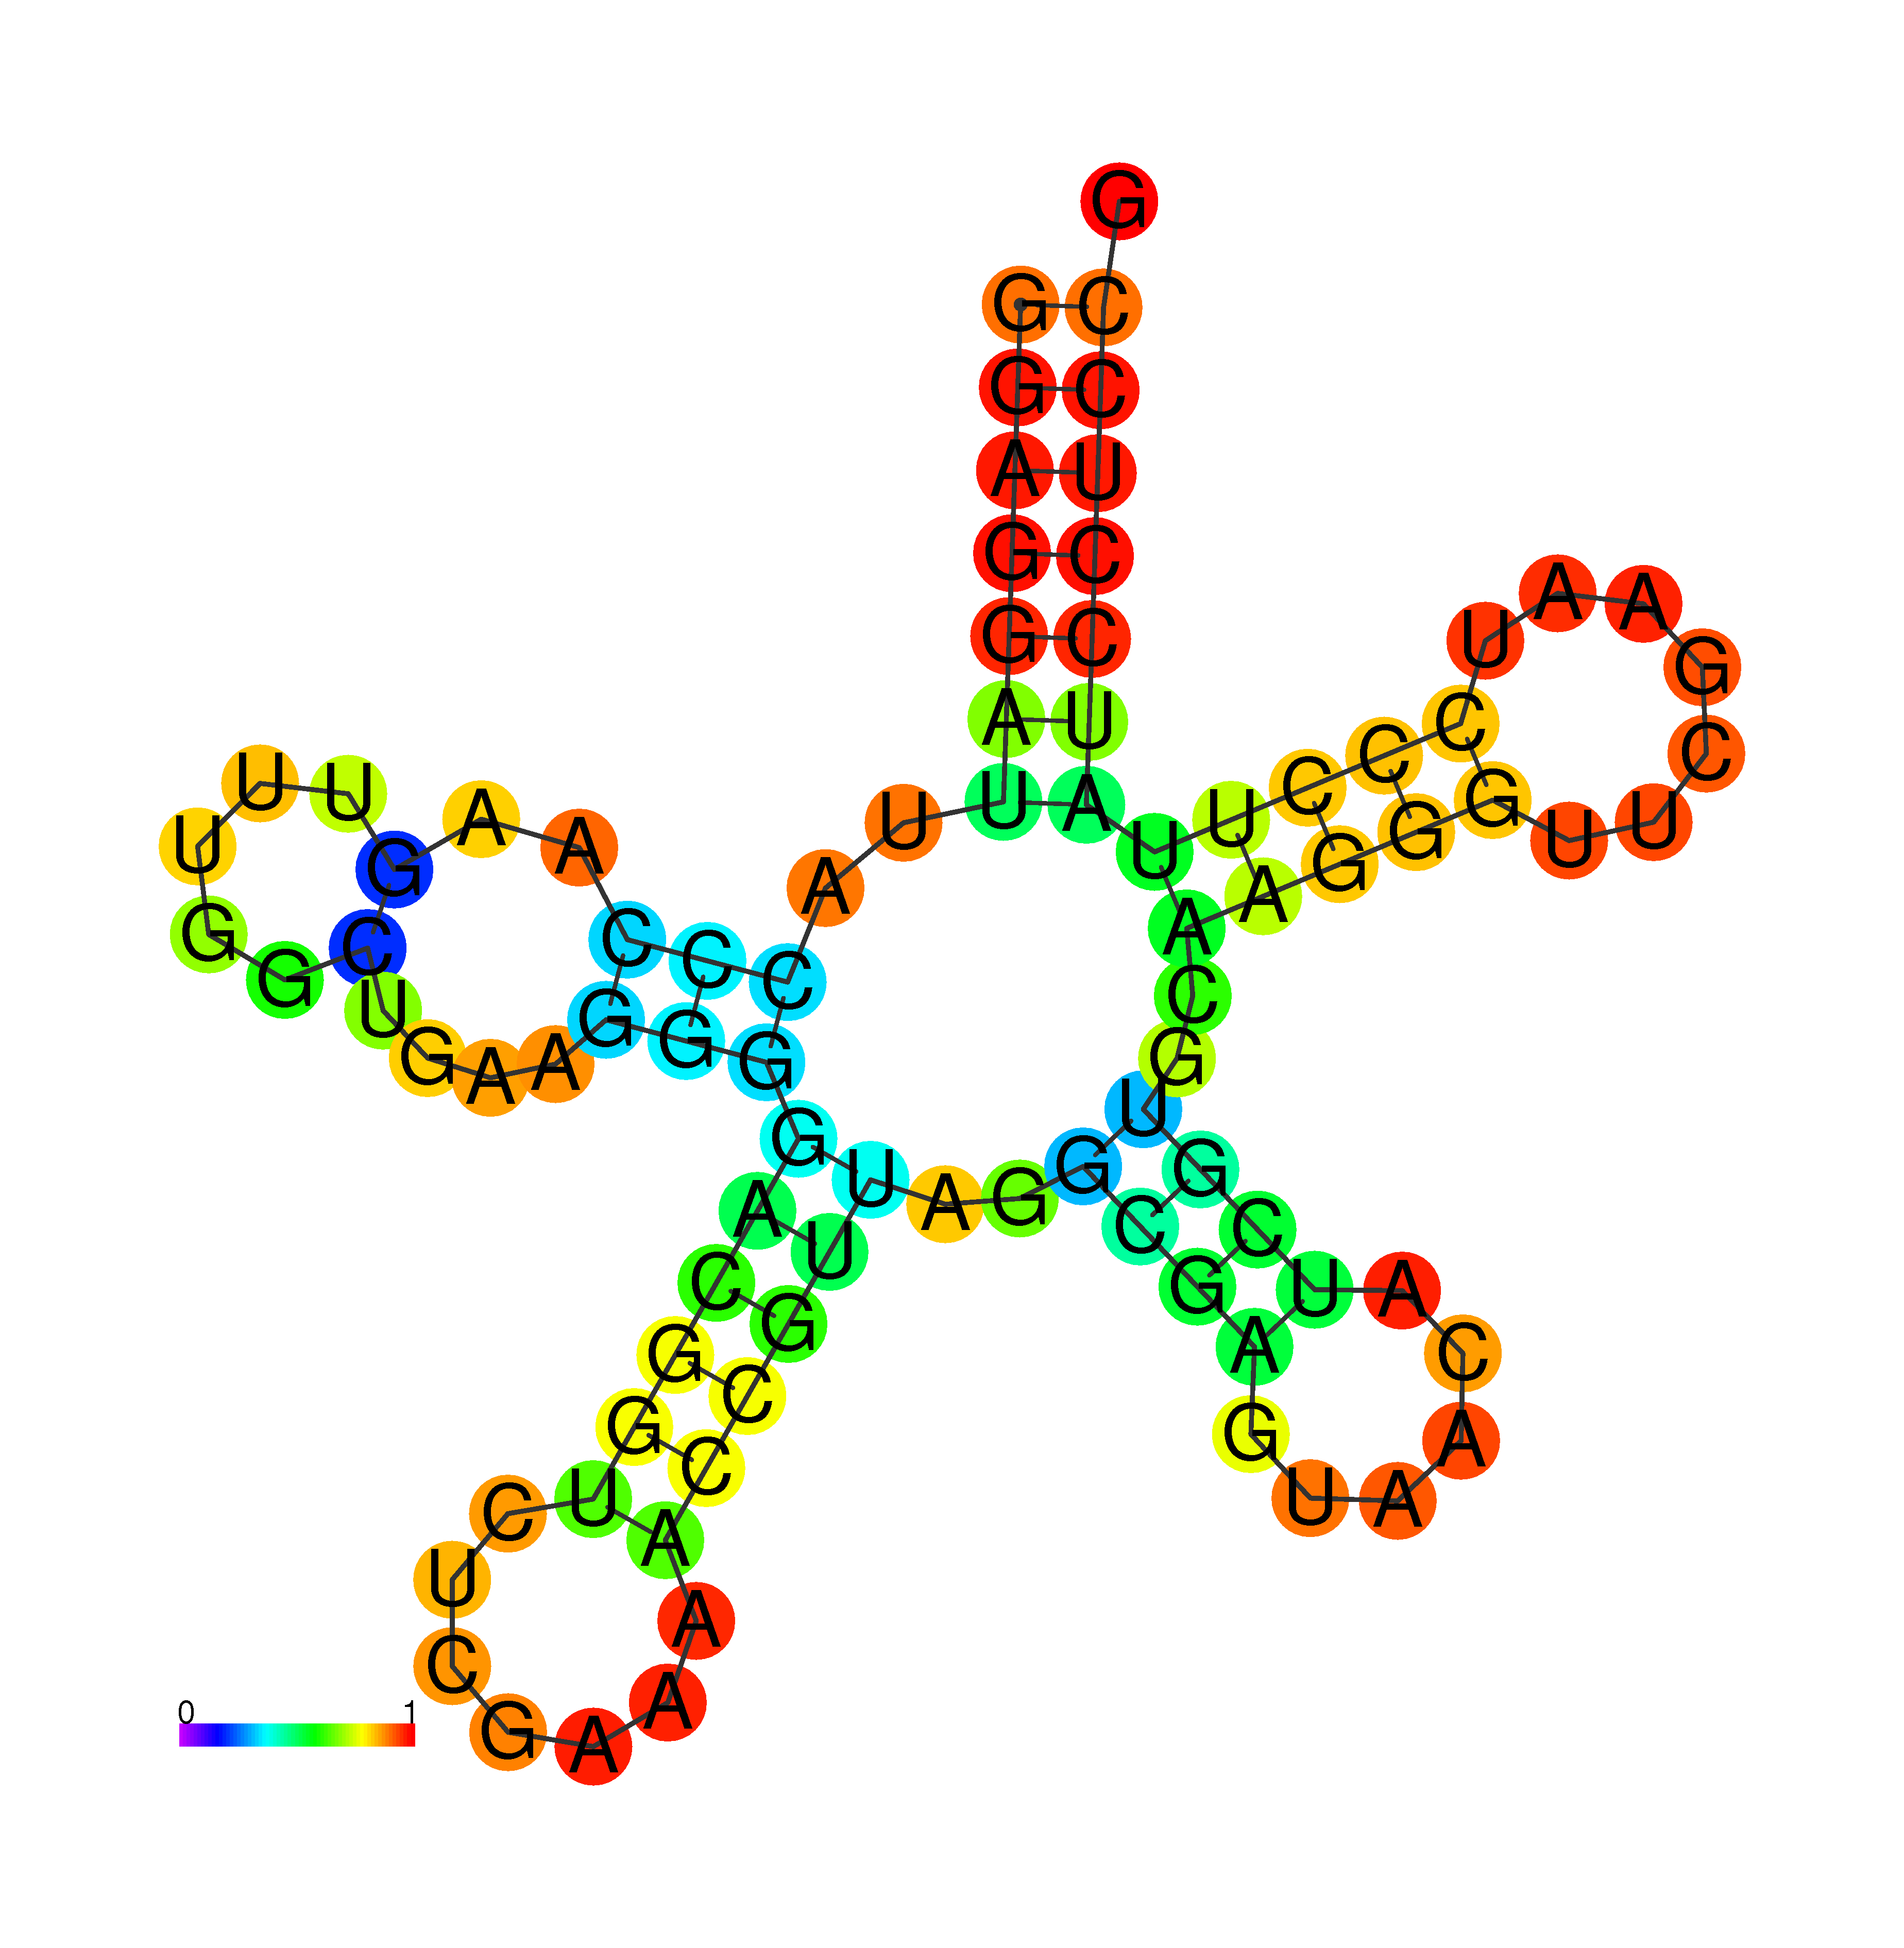
\includegraphics[width=.6\linewidth]{pics/structure.png}}
  \caption{Вторичная структура}
\end{subfigure}%
\begin{subfigure}{.3\textwidth}
  \centering
  \fbox{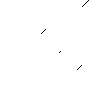
\includegraphics[width=.6\linewidth]{pics/etalon.png}}
  \caption{Матрица контактов}
\end{subfigure}
\begin{subfigure}{.3\textwidth}
  \centering
  \fbox{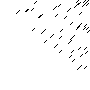
\includegraphics[width=.6\linewidth]{pics/parsed.png}}
  \caption{Матрица разбора}
\end{subfigure}%
\end{figure}
\end{frame}


\begin{frame}{Предсказание вторичной структуры РНК}

\textbf{Где найти эталонные вторичные структуры?}
\begin{itemize}
    \item Выгрузить из биологических баз данных
    \item Сгенерировать некоторым тулом
\end{itemize}

\vspace{6mm}

\textbf{Проблема:} в базах слишком мало данных для обучения
\vspace{1mm}

\textbf{Решение:} transfer learning --- обучить нейросеть на сгенерированных данных, а затем дообучить ее на реальных вторичных структурах

\vspace{6mm}

\textbf{Проблема:} не хотим эмулировать работу уже существующего тула и повторять его ошибки
\vspace{1mm}

\textbf{Решение:} обучить n сетей для n тулов, а при дообучении на реальных данных соединить результаты в общую модель

\end{frame}

\begin{frame}{Предсказание вторичной структуры РНК}
\textbf{Задачи:}  
\begin{itemize}
    \item Предсказание вторичных структур тРНК по сгенерированным различными инструментыми данным
    \item Предсказание реальных вторичных структур цепочек тРНК
\end{itemize} 

\vspace{6mm}

\textbf{Технологии и данные}
\begin{itemize}
    \item Платформа YaccConstructor
    \item Библиотека Keras и фреймворк Tensorflow
    \item Инструменты HotKnots, pknotsRG, RNAstructure и SPOT-RNA
    \item Базы данных RNAcentral, Pseudobase и RNAstrand 
\end{itemize}

\vspace{6mm}

\end{frame}


\begin{frame}{Используемые инструменты}
\setlength\tabcolsep{1pt}
\begin{tabular}{cl}  
    \parbox{0.6\linewidth}{
        Требования
        \begin{itemize}
            \item Основаны на разных алгоритмах
            \item Результаты различаются, но все имеют высокую точность
            \item Удобство и скорость работы
            \item Предсказывают псевдоузлы
        \end{itemize}
    }
    & \begin{tabular}{l}
    
        \vspace{-4mm}
        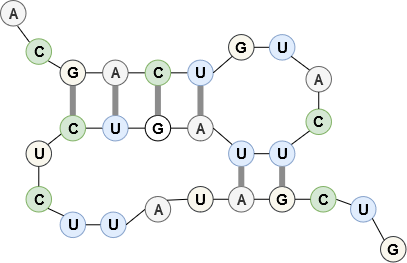
\includegraphics[width=4.5cm]{pics/pseudoknot.png}
    \end{tabular}  \\
\end{tabular}

\vspace{6mm}
        Выбрали
        \begin{itemize}
            \item HotKnots --- эвристический алгоритм + MFE
            \item SPOT-RNA --- deep learning
            \item pknotsRG --- Turner energy rules + MFE
            \item RNAstructure --- динамическое программирование + MFE
         \end{itemize} 
\end{frame}


\begin{frame}{Нейронная сеть: этап 1}

\setlength\tabcolsep{0.1pt}
\begin{tabular}{cl}  
    \parbox{0.85\linewidth}{
        \begin{itemize}
            \item ResNet из десяти блоков для каждого из четырех тулов
            \item Loss --- взвешенная попиксельная разница
            %\vspace{5mm\onelineskip}
             \item Метрики
            \begin{itemize}
                \item Precision --- сколько из предсказанных контактов действительно являются контактами в эталоне
                \item Recall --- сколько из требуемых контактов найдено
                \item F1 score --- объединяющая метрика
            \end{itemize}
        \item Длина цепочки от 1 до 100, около 18000 образцов на каждую сеть, train:test = 80\%:20\%
        \end{itemize}
    }
    & \begin{tabular}{l}
        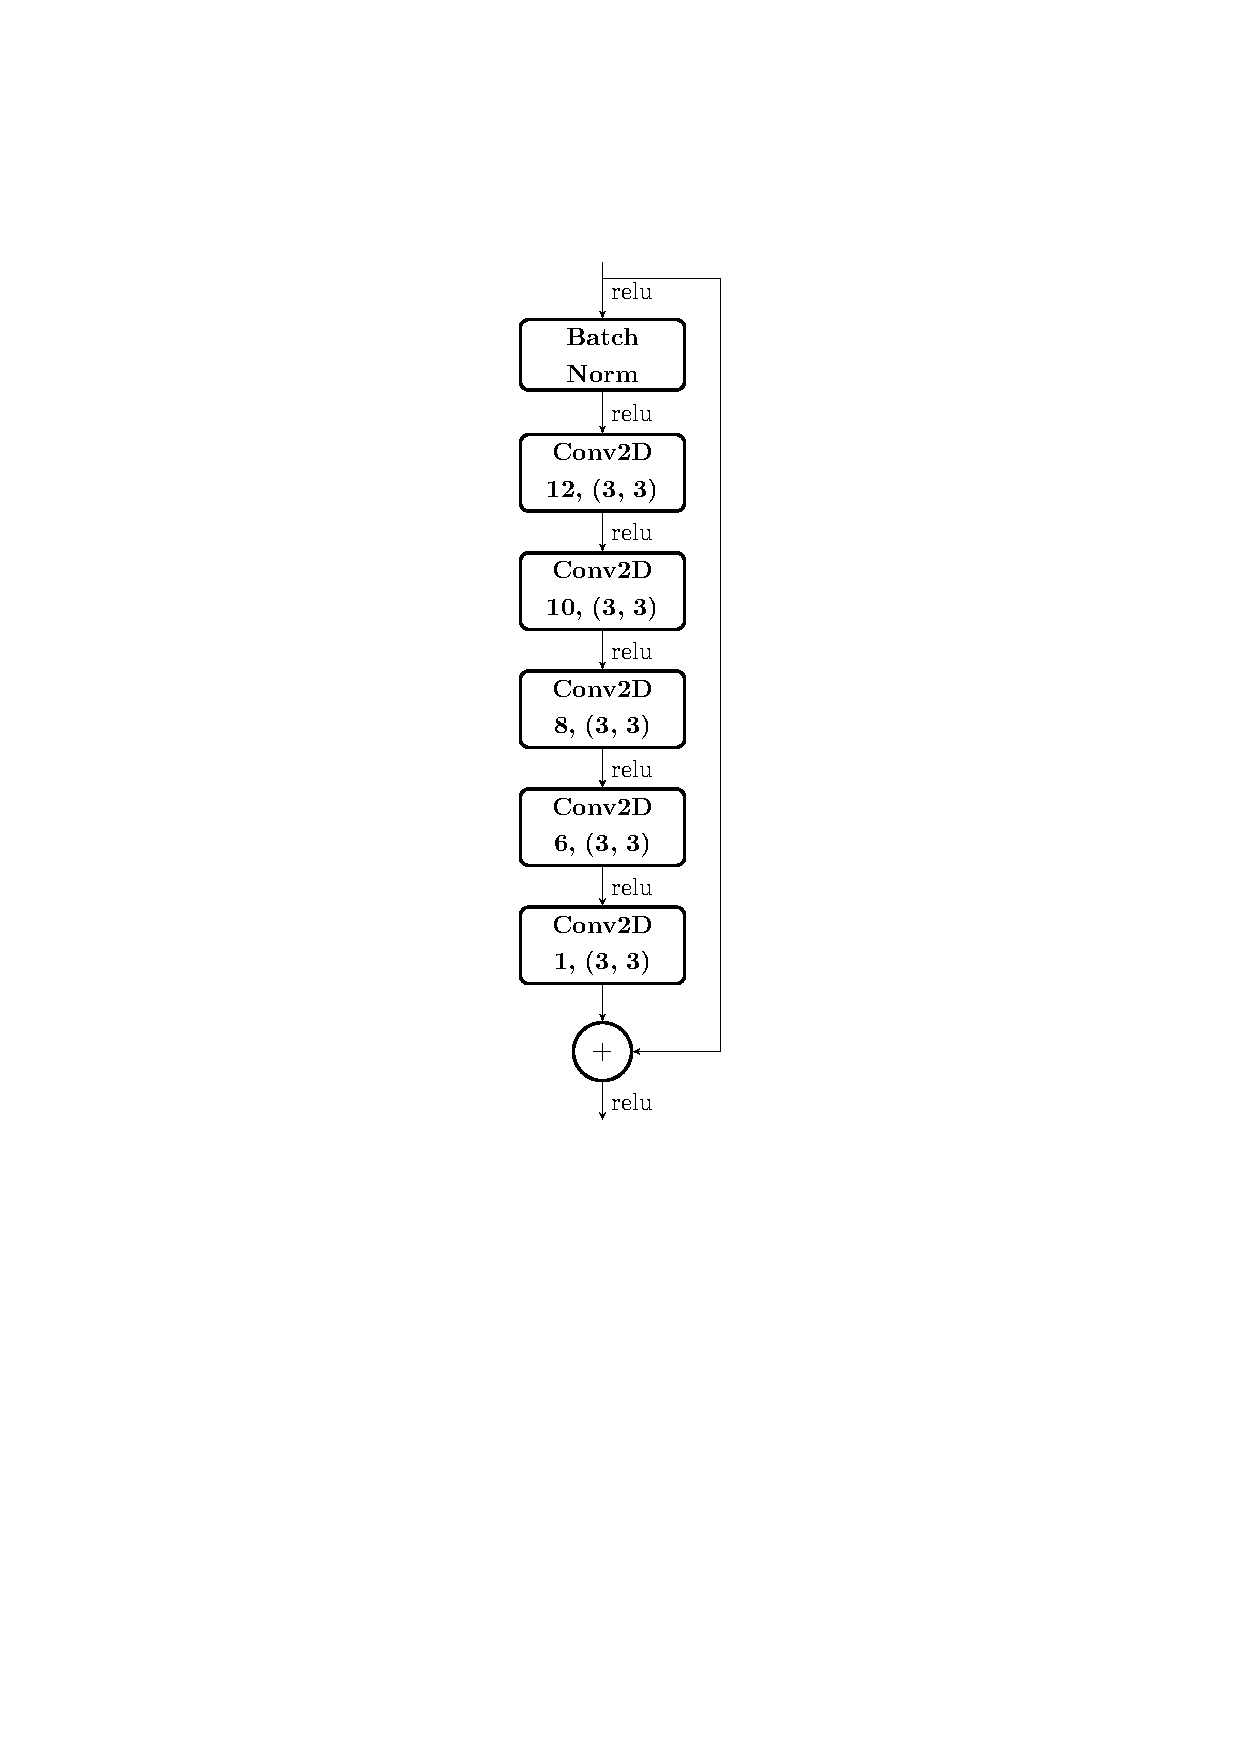
\includegraphics[width=2.0cm]{pics/res_unit.pdf}
    \end{tabular}  \\
\end{tabular}
    
\end{frame}


\begin{frame}{Результаты: этап 1}

Средние значения метрик на тестовых выборках для каждой модели

\vspace{4mm}

\setlength\extrarowheight{4pt}
\begin{table}[h]
\begin{tabular}{|P{2.5cm}|P{2.5cm}|P{2.5cm}|P{2.5cm}|P{2.5cm}|}
\hline
Base tool         & Precision & Recall & F1 score \\ \hline \hline
HotKnots     & 38\%      & 44\%   & 39\%     \\ \hline
pknotsRG     & 40\%      & 45\%   & 40\%     \\ \hline
RNAstructure & 41\%      & 48\%   & 42\%     \\ \hline
SPOT-RNA     & 41\%      & 50\%   & 42\%     \\ \hline
\end{tabular}
\end{table}

\end{frame}


\begin{frame}{Нейронная сеть: этап 2}

\centering
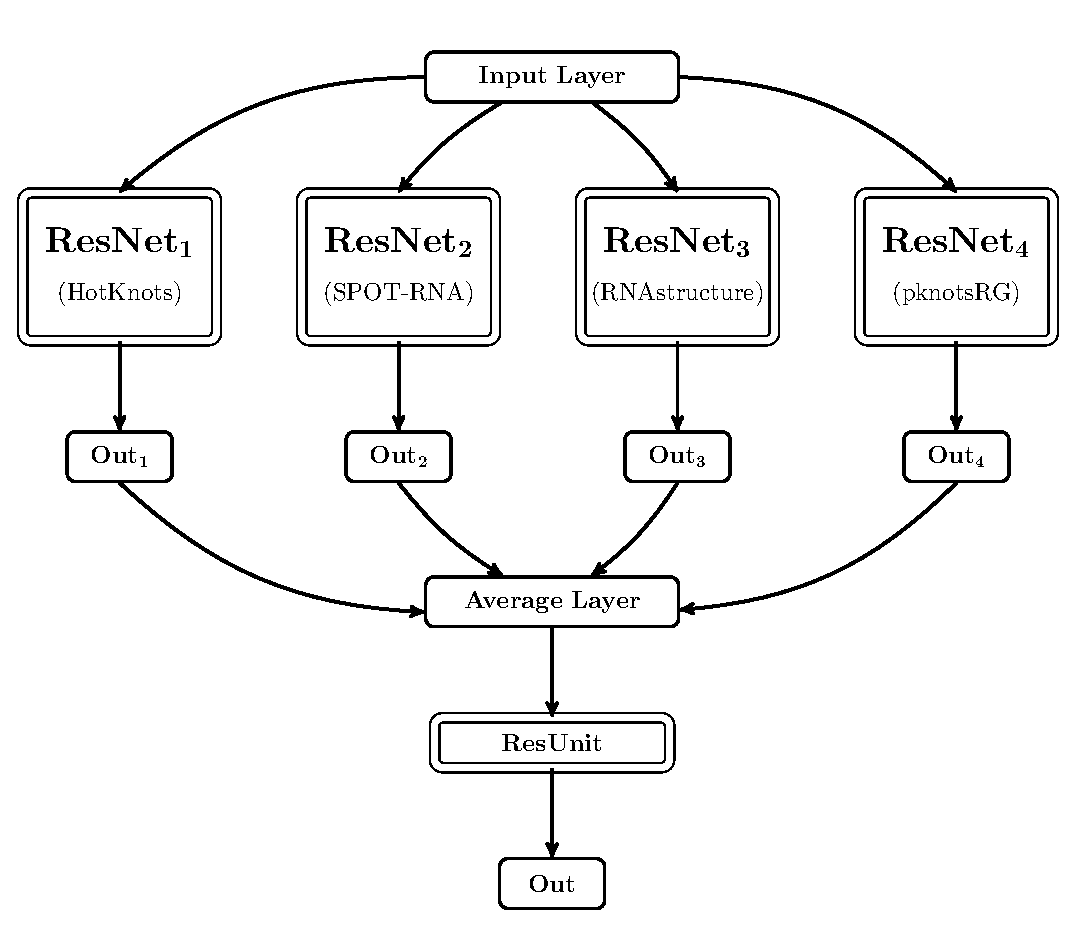
\includegraphics[width=9.0cm]{pics/nn.pdf}

    
\end{frame}


\begin{frame}{Результаты: этап 2}

База Pseudobase --- 255 структур, все с псевдоузлами

\centering
\includegraphics[width=10.5cm]{pics/plot_pb.png}

\end{frame}

\begin{frame}{Результаты: этап 2}

База RNAstrand --- 819 структур, из них 74 с псевдоузлами

\centering
\includegraphics[width=10.5cm]{pics/plot_rs.png}

\end{frame}

\begin{frame}{Итоги}
\textbf{Публикации} 

\begin{itemize}
    \item Semyon Grigorev, Dmitry Kutlenkov, Polina Lunina. Secondary structure prediction by combination of formal grammars and neural networks. BMC Bioinformatics, Scopus
    \item Polina Lunina, Semyon Grigorev. On Secondary Structure Analysis by Using Formal Grammars and Artificial Neural Networks. LNBI, Scopus
\end{itemize}
     

\vspace{6mm}

\textbf{Планы на будущее}
\begin{itemize}
    \item Улучшение полученных результатов
    \item Подготовка к конференции AlCoB 2020\&2021
\end{itemize}

\vspace{6mm}

\end{frame}


\end{document}